\chapter{Theoretische Grundlagen}
Wir verwenden für den Aufbau einer funktonierenden Kommunikation viele verschiedene Arten von Code, Dateiformaten und Übertragungsprotokollen. Ein kleiner Teil des Datenaustauschs ist zur Veranschaulichung hier erklärt.\\\\
% Hier ist was, das wahrscheinlich schon zu praktisch ist, aber wir benutzen keine phys. Formeln o.ä.
% Dashalb regex, ajax, json

% ja, hast recht. kannst einfach noch das machen:
% - Server-Client-Modell
% 	- Aufgaben (siehe server.tex)
%	- Kommunikation (HTTP, ajax)
% 		- Upload
%		- Templates
%		- Static Assets
% - Datenspeicherung (json, xml)
% - Datenkonvertierung (regex)
% - Websicherheit (SSL, hashes)

% Aber wirklich, kann alles ganz kurz gefasst sein.

% Das erklärt jetzt irgendwie den ganzen Datenaustausch, aber ich wollte die Begriffe nicht abstrakt erkären... Das versteht dann kein Mensch mehr // Falls das so überhaupt jemand versteht
Zunächst liegen die Daten als XML-Code vor. In diesem Format werden Daten durch Text dargestellt, welcher mit Tags unterteilt ist. Ein Tag sieht dabei so aus: \texttt{<name> Text </name>}. Schachtelt man nun diese Tags ineinander, kann man relativ leicht Datenstrukturen darstellen. Auf XML, \texttt{e\textbf{X}tended \textbf{M}arkup \textbf{L}anguage} basiert \HTML, \texttt{\textbf{H}yper\textbf{T}ext \textbf{M}arkup \textbf{L}anguage}, das dieselbe strukturierende Funktion für Webseiten zur Verfügung stellt. Um sich den Benutzern anzupassen, muss das \HTML vom Server generiert werden. Um alle dies zu erleichtern, wandeln wir den XML-Code in ein anderes Datenformat, JSON, um, da der Server damit besser umgehen kann. Wir haben uns dazu entschieden, für diesen Vorgang \texttt{Regular Expressions}, kurz \texttt{regexp} zu benutzen: Ein Platzhalterstring wird auf eine Quelle \glqq gematcht\grqq , d.h. alle Strings, die auf ein entsprechendes Muster passen, werden mit einer Schlüsselbezeichnung zurückgegeben. So wird der reguläre Ausdruck \url{/^[ \t]*\$/} auf alle nur mit Leerzeichen und Tabs gefüllten Zeilen passen. Damit lassen sich verschachtelte Klassenangaben wie bsp. \texttt{10A/ 10ABCET1} auftrennen: die Ethikgruppe 1 der Klassen 10a, 10b und 10c ist hier gemeint.\\

Der XML-Code wird so Schritt für Schritt in eine JSON-Datei (\texttt{JavaScript Object Notation}) umgewandelt. Dieses weit verbreitete Speicherformat stellt Daten als Schlüssel und Werte dar, die durch Listen und Gruppen strukturiert sind.\\

Die ursprüngliche Quelle für das XML-Dokument liegt hier bei einem Stundenplanverwaltungsprogramm der Schule. Die dort generierten Dateien werden über die \url{/upload} Webseite hochgeladen. Dafür werden jQuery und AJaX verwendet. jQuery ist eine beliebte JavaScript Bibliothek, die dem Anwender viel Arbeit wie das manuelle Registrieren von EventListenern, die unter anderem für das Abfangen von Mausbewegungen oder Tastendrücken sorgen können, erspart. AJaX steht für \glqq Asynchronous JavaScript and XML\grqq\  und bedeutet, dass über JavaScript die Seite mit dem Server kommunizieren kann, ohne eine komplette HTML-Seite als Rahmen zu übermitteln. Damit können sämtliche Dateien problemlos auf den Server übertragen werden.\\

Nach dem Hochladen und dem Konvertieren sind die Dateien bereit, vom Client abgerufen zu werden. Dafür müssen sie in einen von einem Browser interpretierbaren Code umgewandelt werden, was in fast allen Fällen HTML, also \texttt{Hypertext Markup Language} ist. Dafür benutzen wir den Template-Parser von Pyramid, einem Serverframework. Es werden in einem HTML-Dokument Angaben gemacht, die vom Server mit entsprechenden Informationen ersetzt werden. Dabei wird das zuvor generierte JSON-Dokument verwendet.\\

Zusammen mit Stildateien und Scriptcode werden die Informationen an den Client übertragen. Dafür muss dieser zunächst ein Passwort angeben. Noch auf der Clientseite wird daraus eine Prüfsumme erstellt, aus der das ursprüngliche Passwort mit aktuellen technischen Möglichkeiten nicht ableitbar ist. Diese wird auch als \texttt{Hashsum} bezeichnet, was so viel wie \glqq zerhackter Wert \grqq\  bedeutet. Ein solcher wird mithilfe eines Requests an den Server übertragen, der die Prüfsumme mit einer Liste vergleicht und eine positive oder negative Rückmeldung an den Client sendet.\\

Vor dem Auslesen des Passworts ist der Kommunikationsweg zwischen Server und Client sicher, doch ein weiteres Risiko bleibt bestehen: Wer den Hashwert abfängt, kann sich als Client ausgeben und diesen direkt übertragen. Die einzige Lösung dagegen ist, den kompletten Datenaustausch End-to-End zu verschlüsseln. Eine Lösung hierfür ist SSL, welches durch ein etwas  anderes Protokoll, \texttt{https} statt \texttt{http}, genau dies gewährleistet.

\begin{figure}[ht]
	\centering
  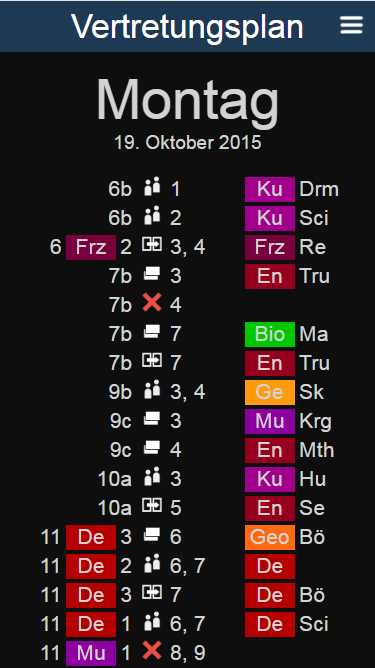
\includegraphics[height=10cm]{mobile.png}
	\caption{Screenshot der Seite}
	\label{fig1}
\end{figure}
